\documentclass[a4paper, 12pt]{article}
\usepackage[top=2cm, bottom=2cm, left=2.5cm, right=2.5cm]{geometry}
\usepackage[utf8]{inputenc}
\usepackage{amsmath, amsfonts, amssymb}
\usepackage{float}
\usepackage{graphicx}
\usepackage[brazil]{babel}
\usepackage{indentfirst}

\title{Titulo do Trabalho.}
\author{Nome do autor \\ email@email.com}
\date{16/04/2017}

\begin{document}
\maketitle \newpage

\tableofcontents \newpage

\listoffigures \newpage

\listoftables \newpage


\section{Introdução}
Aqui vem o texto Aqui vem o texto Aqui vem o texto Aqui vem o texto Aqui vem o texto 
Aqui vem o texto Aqui vem o texto Aqui vem o texto Aqui vem o texto Aqui vem o texto 
Aqui vem o texto Aqui vem o texto Aqui vem o texto Aqui vem o texto Aqui vem o texto 
Aqui vem o texto Aqui vem o texto Aqui vem o texto Aqui vem o texto Aqui vem o texto 
Aqui vem o texto Aqui vem o texto Aqui vem o texto Aqui vem o texto Aqui vem o texto 
Aqui vem o texto Aqui vem o texto Aqui vem o texto Aqui vem o texto Aqui vem o texto 
\begin{figure}[htb]
	\centering
	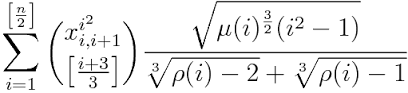
\includegraphics[scale=0.4]{Imagens/funcao.png}
	\caption{Função matemática}
	\label{figur}
\end{figure}

Aqui vem o texto Aqui vem o texto Aqui vem o texto Aqui vem o texto Aqui vem o texto 
Aqui vem o texto Aqui vem o texto Aqui vem o texto Aqui vem o texto Aqui vem o texto 
Aqui vem o texto Aqui vem o texto Aqui vem o texto Aqui vem o texto Aqui vem o texto 
Aqui vem o texto Aqui vem o texto Aqui vem o texto Aqui vem o texto Aqui vem o texto\cite{meuatalhoref} 

Aqui vem o texto Aqui vem o texto Aqui vem o texto Aqui vem o texto Aqui vem o texto 
Aqui vem o texto Aqui vem o texto Aqui vem o texto Aqui vem o texto Aqui vem o texto 
Aqui vem o texto Aqui vem o texto Aqui vem o texto Aqui vem o texto Aqui vem o texto 
Aqui vem o texto Aqui vem o texto Aqui vem o texto Aqui vem o texto Aqui vem o texto 


\section{Desenvolvimento}
Aqui vem o texto Aqui vem o texto Aqui vem o texto Aqui vem o texto Aqui vem o texto 
Aqui vem o texto Aqui vem o texto Aqui vem o texto Aqui vem o texto Aqui vem o texto 
Aqui vem o texto Aqui vem o texto Aqui vem o texto Aqui vem o texto Aqui vem o texto 
Aqui vem o texto Aqui vem o texto Aqui vem o texto Aqui vem o texto Aqui vem o texto 
Aqui vem o texto Aqui vem o texto Aqui vem o texto Aqui vem o texto Aqui vem o texto 
Aqui vem o texto Aqui vem o texto Aqui vem o texto Aqui vem o texto Aqui vem o texto 

\begin{table}
	\centering
	\begin{tabular}{|c|c|}
		teste 1 & teste 2\\
		teste 1 & teste 2\\
		teste 1 & teste 2\\
		teste 1 & teste 2\\
	
	\end{tabular}
	\caption{Tabela Teste}
	\label{tabela-teste}
\end{table}

Aqui vem o texto Aqui vem o texto Aqui vem o texto Aqui vem o texto Aqui vem o texto 
Aqui vem o texto Aqui vem o texto Aqui vem o texto Aqui vem o texto Aqui vem o texto 
Aqui vem o texto Aqui vem o texto Aqui vem o texto Aqui vem o texto Aqui vem o texto 
Aqui vem o texto Aqui vem o texto Aqui vem o texto Aqui vem o texto Aqui vem o texto\cite{meuatalhoArticle} 
\subsection{Sub Desenvolvimento}
Aqui vem o texto Aqui vem o texto Aqui vem o texto Aqui vem o texto Aqui vem o texto 
Aqui vem o texto Aqui vem o texto Aqui vem o texto Aqui vem o texto Aqui vem o texto 
Aqui vem o texto Aqui vem o texto Aqui vem o texto Aqui vem o texto Aqui vem o texto 
Aqui vem o texto Aqui vem o texto Aqui vem o texto Aqui vem o texto Aqui vem o texto 

\begin{figure}[htb]
	\centering
	
\includegraphics[scale=0.4]{Imagens/latex.png}
	\caption{\LaTeX é o futuro.}
	\label{latec_figure}
\end{figure}

\subsubsection{Sub Sub seção}
Aqui vem o texto Aqui vem o texto Aqui vem o texto Aqui vem o texto Aqui vem o texto 
Aqui vem o texto Aqui vem o texto Aqui vem o texto Aqui vem o texto Aqui vem o texto 
Aqui vem o texto Aqui vem o texto Aqui vem o texto Aqui vem o texto Aqui vem o texto 
Aqui vem o texto Aqui vem o texto Aqui vem o texto Aqui vem o texto Aqui vem o texto 

\begin{table}
	\centering
	\begin{tabular}{|c|c|}
		teste 1 & teste 2\\
		teste 1 & teste 2\\
		teste 1 & teste 2\\
		teste 1 & teste 2\\
	
	\end{tabular}
	\caption{Tabela Louca}
	\label{tabela-louca}
\end{table}

\newpage
\bibliographystyle{plain} 
\addcontentsline{toc}{section}{Referências}
\bibliography{referencia.bib}

\end{document}












